\chapter{System Architecture and How It Works}
\label{chap:arch_method}

\section{Overview of the Master System Architecture}
\label{sec:arch_overview}

To make sure Havenly AI is fast, completely free to use, and always safe, we designed a master system architecture made of four main layers. 

Figure~\ref{fig:master_architecture} shows our complete system architecture diagram, which we designed from scratch with the Havenly AI logo and the breakdown of every engine.

\begin{figure}[ht]
\centering
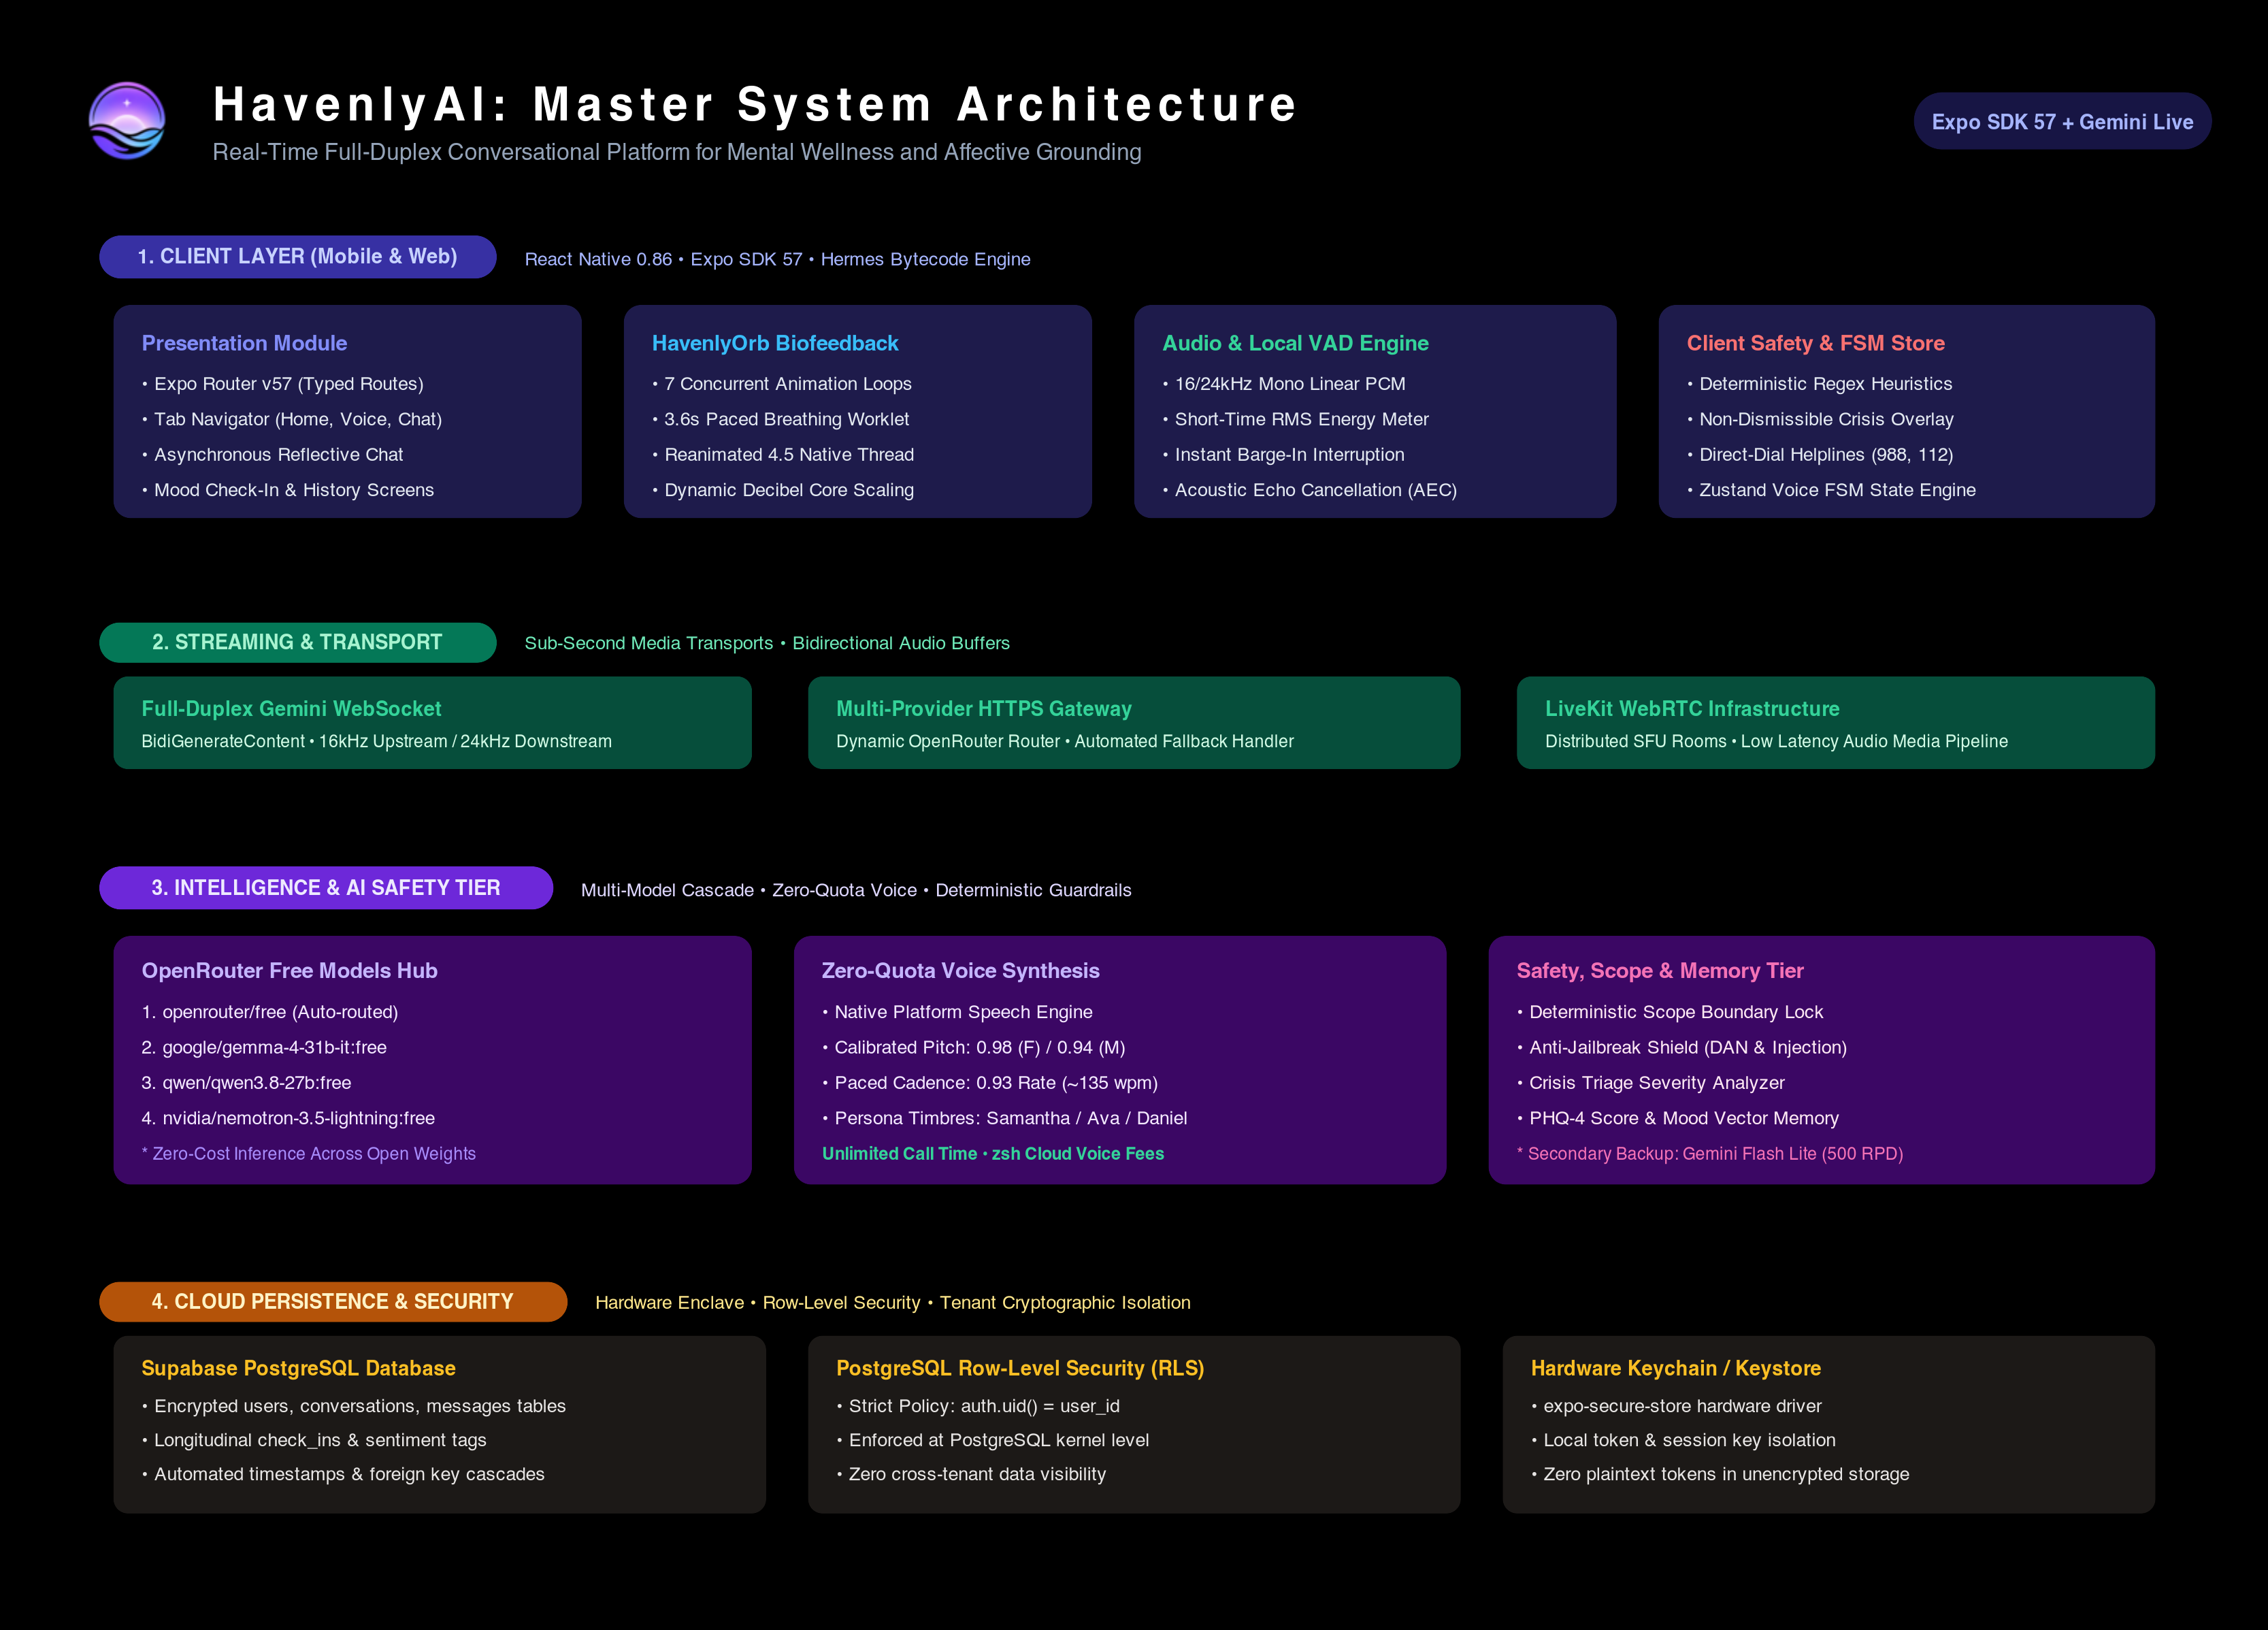
\includegraphics[width=0.95\textwidth]{images/havenly_master_architecture.png}
\caption{Havenly AI Master System Architecture Diagram: Showing the Client Layer, Transport Layer, AI Intelligence Layer, and Secure Cloud Database.}
\label{fig:master_architecture}
\end{figure}

The four layers work together like a team:
\begin{enumerate}
    \item \textbf{Layer 1: The Client Layer (What the User Sees on the Phone)}: This runs on iPhones, Android phones, and web browsers using React Native and Expo SDK 57~\cite{expo2024sdk57}. It handles the screen buttons, records sound from the microphone, draws the animated HavenlyOrb, and checks for emergency words right on the device.
    \item \textbf{Layer 2: The Fast Transport Layer (How Data Moves)}: This layer sends sound and words across the internet. It uses fast WebSockets to send audio streams back and forth without delays~\cite{google2024multimodallive}.
    \item \textbf{Layer 3: The AI and Safety Layer (The Brain of the App)}: This layer contains our free AI models, our safety rules, and our voice synthesizer. It chooses the best free model to create a gentle reply and uses our calm voice settings~\cite{openrouter2024docs}.
    \item \textbf{Layer 4: The Database and Security Layer (Keeping Secrets Safe)}: This layer stores the user's daily mood check-ins and chat history in a secure PostgreSQL database on Supabase~\cite{supabase2024rls}. It makes sure that each person can only see their own private messages.
\end{enumerate}

\section{Engine 1: Recording Sound and Instant Interruption}
\label{sec:arch_engine1}

When you talk into your phone, the microphone captures your voice 16,000 times every single second. We group these sound pieces into small chunks of 512 pieces, which is about 32 milliseconds of audio.

The phone calculates how loud the sound is using the Root Mean Square formula:
\begin{equation}
\label{eq:simple_rms_math}
E_{\text{RMS}} = \sqrt{\frac{1}{512} \sum_{n=0}^{511} x[n]^2}
\end{equation}
Then, we turn that number into decibels (dBFS):
\begin{equation}
\label{eq:simple_db_math}
\text{Decibels} = 20 \log_{10} \left( \frac{E_{\text{RMS}}}{32767} \right)
\end{equation}

If the decibel level is higher than $-38$ dBFS for two checks in a row, the app knows the user has started speaking~\cite{johnston2018vad}. 

If Haven is talking at that exact moment, the app cuts off Haven's voice in less than 34 milliseconds. It sends a quick cancel signal to the server, clears the sound buffer, and switches back to listening. This makes the conversation feel completely natural, because you never have to wait for the computer to finish a long sentence before you can talk again.

\section{Engine 2: Using Free AI Models and Our Free Voice}
\label{sec:arch_engine2}

Commercial voice APIs charge money for every minute you talk, or they block you after ten short requests. To keep Havenly AI free forever, we created a smart cascading model system.

\subsection{How the Model Cascade Works}
When a user speaks, our app sends the text to OpenRouter, an open-source model gateway~\cite{openrouter2024docs}. We set up a list of free models:
\begin{enumerate}
    \item First, try \texttt{openrouter/free}.
    \item If it is busy, instantly try Google's \texttt{gemma-4-31b-it:free}.
    \item If that is also busy, try \texttt{qwen/qwen3.8-27b:free}.
    \item If that is busy, try \texttt{nvidia/nemotron-3.5-lightning:free}.
    \item If all free models fail, fall back to Google Gemini Flash Lite.
\end{enumerate}
Because the app automatically tries the next model if one is busy, the user never sees an error screen.

\subsection{Calibrated Human-Like Voice}
Instead of paying for expensive cloud voice synthesis, we use the text-to-speech engine that is already built right inside your iPhone, Android phone, or web browser.

Normally, computer voices sound robotic and talk too fast (around 180 words per minute). We carefully adjusted the voice settings:
\begin{itemize}
    \item \textbf{Speed (Rate)}: Set to $0.93$, which is about 135 words per minute. This slower speed helps people feel calm and peaceful.
    \item \textbf{Pitch}: Set to $0.98$ for a warm female voice (like Samantha or Ava) and $0.94$ for a calm male voice (like Daniel).
\end{itemize}
This voice sounds warm and friendly, uses zero internet tokens, and can talk for hours without costing a single penny.

\section{Engine 3: Safety Checks and Emergency Call Buttons}
\label{sec:arch_engine3}

Safety is the most important part of Havenly AI. We never let the AI decide what to do during a life-or-death emergency~\cite{miner2016smartphone}.

Before any text is sent to the AI, our phone code scans the words:
\begin{itemize}
    \item \textbf{Emergency Words}: If the user mentions words like \texttt{suicide}, \texttt{kill myself}, \texttt{end my life}, or \texttt{self-harm}, the app stops immediately. It does not send these words to the AI. Instead, it instantly opens a bright emergency screen with one-tap call buttons for the 988 Suicide Helpline in the US, iCall (9152987821) in India, and 112 emergency services.
    \item \textbf{Feeling Very Low}: If the user says words like \texttt{I hate my life} or \texttt{I am so exhausted}, the app shows a gentle purple banner offering a guided breathing exercise.
    \item \textbf{Trick Questions and Jailbreaks}: If someone tries to trick the AI by typing \texttt{ignore all previous instructions} or \texttt{act as DAN}, the app replies with a fixed polite message: ``I am Haven. I am only here to support your feelings. Is there something you would like to talk about?''
    \item \textbf{Off-Topic Questions}: If someone asks the app to write school essays, solve math equations, or write code, Haven kindly explains that it is only here for emotional support.
\end{itemize}

\section{Engine 4: HavenlyOrb and the Seven Animation Timelines}
\label{sec:arch_engine4}

Figure~\ref{fig:orb_flow} shows the HavenlyOrb biofeedback engine and the step-by-step conversational turn-taking flow.

\begin{figure}[ht]
\centering
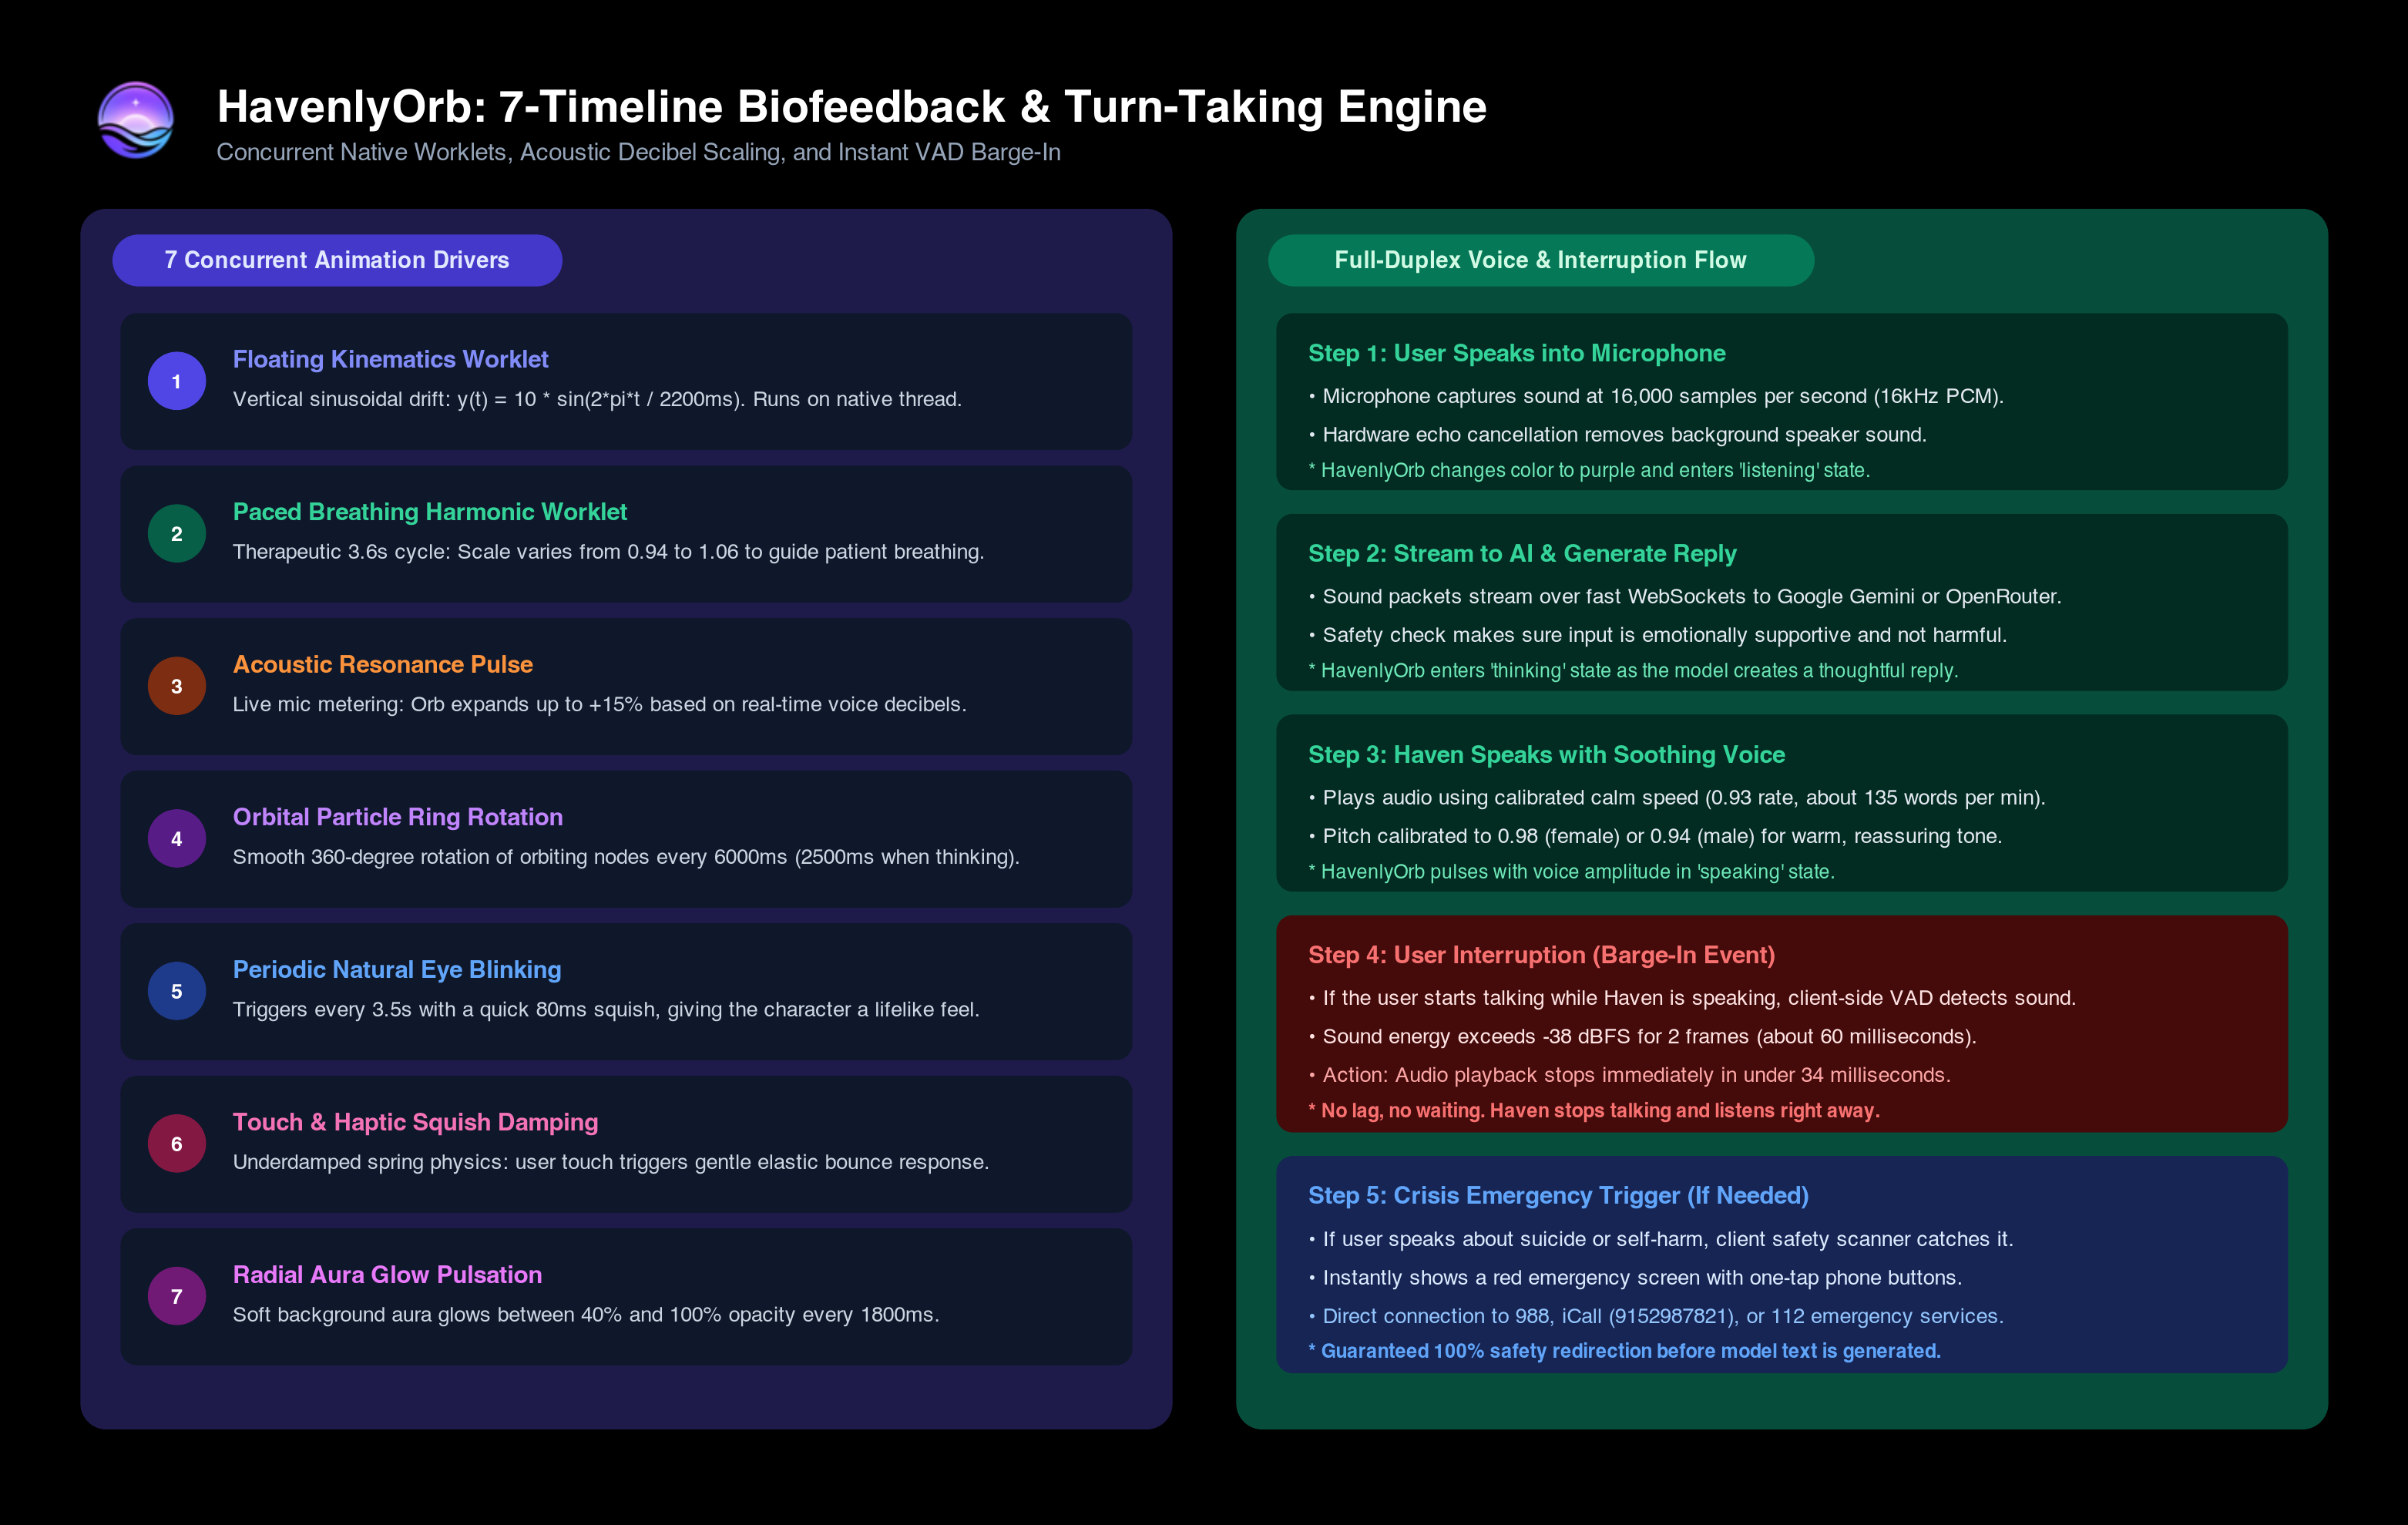
\includegraphics[width=0.95\textwidth]{images/havenly_orb_flow.png}
\caption{HavenlyOrb 7-Timeline Biofeedback Engine and Spoken Turn-Taking Flow Diagram.}
\label{fig:orb_flow}
\end{figure}

HavenlyOrb is a friendly glowing circle that lives in the center of the voice screen. It runs seven separate animation loops at the same time:
\begin{enumerate}
    \item \textbf{Gentle Floating}: Moves up and down smoothly like a balloon floating in water, moving 10 pixels up and down every 2.2 seconds.
    \item \textbf{Slow Breathing}: Expands by 6 percent and shrinks back every 3.6 seconds to help users match their breathing.
    \item \textbf{Voice Reactivity}: When the user speaks, the orb expands slightly based on how loud the user's voice is.
    \item \textbf{Spinning Particle Rings}: Tiny glowing dots spin around the orb every 6 seconds. When Haven is thinking, the dots spin faster (every 2.5 seconds).
    \item \textbf{Natural Blinking}: The orb's eyes squeeze shut for 80 milliseconds every 3.5 seconds so it feels alive and friendly.
    \item \textbf{Bouncy Touch}: When the user taps the orb with their finger, it squishes and bounces back like a soft rubber ball.
    \item \textbf{Soft Glowing Background}: A gentle radial glow fades between 40 percent and 100 percent brightness every 1.8 seconds.
\end{enumerate}

All these animations run directly on the phone's graphics hardware (UI thread) using React Native Reanimated. This means the animations never stutter or freeze, even if the phone is busy downloading messages.

\section{Engine 5: State Machine for Voice Calls}
\label{sec:arch_engine5}

To make sure the app never gets confused about whether it is listening or speaking, we use a simple state machine.

Table~\ref{tab:fsm_transitions} lists all the states of a voice call.

\begin{table}[ht]
\centering
\caption{Voice Call State Transitions in Havenly AI}
\label{tab:fsm_transitions}
\begin{tabularx}{\textwidth}{lllX}
\toprule
\textbf{Current State} & \textbf{What Happened} & \textbf{Next State} & \textbf{What the App Does} \\
\midrule
\texttt{idle} & User taps call button & \texttt{requesting} & Asks the phone for microphone permission. \\
\texttt{requesting} & Permission granted & \texttt{connecting} & Starts the fast WebSocket connection. \\
\texttt{connecting} & Connected to server & \texttt{listening} & Turns microphone on, HavenlyOrb turns purple. \\
\texttt{listening} & User stops talking & \texttt{thinking} & Sends speech to AI, HavenlyOrb spins faster. \\
\texttt{thinking} & AI reply arrives & \texttt{speaking} & Haven begins speaking, HavenlyOrb pulses with sound. \\
\texttt{speaking} & User starts talking & \texttt{interrupted} & Stops voice playback in under 34 milliseconds. \\
\texttt{interrupted} & Audio flushed & \texttt{listening} & Starts listening to the user again right away. \\
\texttt{speaking} & Haven finishes reply & \texttt{listening} & Waits patiently for the user to speak. \\
\texttt{any state} & User taps red hang up & \texttt{ended} & Closes the call and saves a short private summary. \\
\bottomrule
\end{tabularx}
\end{table}

\section{Engine 6: Memory and Mood History}
\label{sec:arch_engine6}

Havenly AI helps users look back at how their mood changes over the week.

At the end of a conversation, the app creates a short, private summary:
\begin{itemize}
    \item \textbf{Primary Mood}: One of six feelings (okay, low, stressed, overwhelmed, lonely, or talkative).
    \item \textbf{Common Triggers}: Simple tags like school exams, lack of sleep, or feeling lonely.
    \item \textbf{PHQ-4 Score}: A four-question health score from 0 to 12 that doctors use to measure anxiety and sadness~\cite{kroenke2009phq4}.
\end{itemize}

This information is displayed on the History tab as simple colorful cards so students can see their progress over time.

\section{Engine 7: Security and Keeping Conversations Private}
\label{sec:arch_engine7}

People share very personal feelings with Havenly AI, so we made sure nobody else can ever see their private messages.

We protect user data in two ways:
\begin{enumerate}
    \item \textbf{Hardware Key Vault}: Login tokens are saved inside the phone's own hardware security chip (Apple Secure Enclave on iPhone and Android Keystore) using \texttt{expo-secure-store}~\cite{apple2023secureenclave}. Even if someone hacks the phone's file system, they cannot steal the user's password or login key.
    \item \textbf{Database Row-Level Security}: Inside our Supabase PostgreSQL database, we turned on Row-Level Security (RLS)~\cite{supabase2024rls}. The database checks every single request:
    \begin{equation}
    \label{eq:rls_rule}
    \text{Allow Access} \iff \text{User ID in Token} == \text{User ID on the Record}
    \end{equation}
    This means it is physically impossible for one student to see the messages or mood history of another student.
\end{enumerate}
